\documentclass[11pt]{article}
\usepackage[margin=1in]{geometry}
\usepackage{graphicx}
\usepackage{booktabs}
\usepackage{tabularx}
\usepackage{array}
\usepackage{float}
\usepackage{hyperref}
\usepackage{enumitem}
\usepackage{xcolor}

\hypersetup{
  colorlinks=true,
  linkcolor=blue,
  urlcolor=blue
}

\title{Phase 1 Progress Report\\Approach--Docking Integration in a Kinematic RL Stack}
\author{RL Brain Trainer Project}
\date{April 22, 2026}

\begin{document}
\maketitle

\begin{abstract}
This report summarizes the current Phase 1 progress of our approach--docking integration project. At this checkpoint, the project is intentionally still below full completion: the kinematic simulation stack, training pipeline, and deterministic evaluation pipeline are operational, isolated approach and docking policies have measurable progress, but end-to-end switched integration is not yet reliable and the VLM component has not started. Based on the current evidence, the project is approximately 45\%--50\% complete.
\end{abstract}

\section{Phase 1 Status}

The project currently satisfies the main purpose of the Phase 1 checkpoint: the simulation, programming, and environment setup are operational, and we have concrete experimental evidence that the research stack is running end-to-end.

What is already working:
\begin{itemize}[leftmargin=1.5em]
  \item A custom Gymnasium kinematic environment for a 7-DoF arm with deterministic reset, step, reward, and evaluation.
  \item Stable-Baselines3 training entry points for separate approach and dock policies.
  \item Artifact generation for checkpoints, training summaries, deterministic evaluation summaries, and throughput benchmarks.
  \item A switching wrapper and alternating fine-tuning pipeline for approach--dock integration experiments.
  \item Regression tests for the kinematic environment and evaluation pipeline.
\end{itemize}

What is not done yet:
\begin{itemize}[leftmargin=1.5em]
  \item Reliable switched execution from approach into docking on the full fixed evaluation suite.
  \item Stable joint fine-tuning that improves both policies simultaneously.
  \item Any VLM-related design, training, or integration. The VLM part has not started.
\end{itemize}

We have also stayed consistent with the current Phase 1 setup. The work remains kinematic-first, with the same observation/action contract and the same approach--dock decomposition. We did not change the project into a different simulator stack or broaden the task scope in a way that would break continuity for Phase 2.

\section{Current Architecture}

The current architecture is a two-policy kinematic RL stack:
\begin{enumerate}[leftmargin=1.5em]
  \item \textbf{Environment.} A pure forward-kinematics Gymnasium environment updates the joint configuration from normalized joint-delta actions and computes the end-effector pose without contact dynamics, Gazebo physics, or ROS execution in the learning loop.
  \item \textbf{Observation contract.} The policy input is a dictionary observation containing joint position, delta joint state, previous action, goal pose errors, waypoint placeholders, task/mode flags, progress features, and joint-limit margin. This keeps the interface stable for later phases.
  \item \textbf{Approach policy.} The current approach policy is trained with PPO using \texttt{MultiInputPolicy} over 12 parallel environments.
  \item \textbf{Dock policy.} The current dock policy is trained with TD3 using \texttt{MultiInputPolicy}, tighter action limits, and a reverse curriculum that expands outward from local capture to handoff-edge conditions.
  \item \textbf{Integration layer.} A hysteresis-based switcher decides when to leave the approach policy and enter the dock policy based on position error, dwell steps, action magnitude, and regression checks.
\end{enumerate}

In short, the architecture for Phase 1 is not a single monolithic policy. It is a structured two-policy system with a stable kinematic environment and a switching layer.

\section{How We Train the Model}

\subsection{Approach Training}

The approach model is trained as a pose-reaching and handoff-preparation policy. The action is a 7-dimensional normalized joint delta, and the reward emphasizes position progress, light orientation shaping, near-goal bonuses, dwell bonuses, drift penalties, smooth actions, and joint-limit penalties. A representative long-run setup uses:
\begin{itemize}[leftmargin=1.5em]
  \item PPO with \texttt{MultiInputPolicy}
  \item 12 parallel environments on CUDA
  \item 48-step episodes
  \item learning rate \(5 \times 10^{-5}\)
  \item a handoff-ready success threshold of 8 mm with 4 dwell steps
\end{itemize}

\subsection{Dock Training}

The dock model is trained as a local precision controller after the arm reaches the handoff region. The current dock setup uses:
\begin{itemize}[leftmargin=1.5em]
  \item TD3 with \texttt{MultiInputPolicy}
  \item 12 parallel environments on CUDA
  \item 32-step episodes
  \item strict success threshold of 5 mm and 0.05 rad
  \item reverse curriculum stages: \texttt{anchor\_hold}, \texttt{micro\_capture}, \texttt{local\_capture}, and \texttt{handoff\_edge}
\end{itemize}

This curriculum design lets the dock policy first learn local precision, then gradually handle larger residual offsets from the approach policy.

\subsection{Joint Fine-Tuning}

We also built an alternating fine-tuning loop. One cycle first resumes and fine-tunes the approach checkpoint, then fine-tunes the dock checkpoint, and finally evaluates the switched system. This is our current integration training path, but the most recent smoke experiment shows that the co-training balance is still unstable: dock performance can improve while approach performance collapses.

\section{Operational Evidence}

\begin{table}[H]
\centering
\begin{tabularx}{\textwidth}{>{\raggedright\arraybackslash}p{0.26\textwidth} >{\raggedright\arraybackslash}p{0.18\textwidth} X}
\toprule
Evidence item & Result & Why it matters \\
\midrule
Kinematic env + eval tests & 8/8 passed & Confirms reset/step logic, observation contract, deterministic evaluation suite, and summary generation are working. \\
16-env PPO smoke benchmark & 1761.7 steps/s on CPU, 1790.3 steps/s on GPU & Shows the simulation/training stack is operational with parallel rollout throughput. \\
TD3 parallel smoke benchmark & 272.0 \(\rightarrow\) 883.1 \(\rightarrow\) 1657.6 steps/s from 1/4/8 envs & Confirms parallel vectorized training is functioning and scaling as intended. \\
Training artifacts & Checkpoints, \texttt{training\_summary.json}, \texttt{eval\_summary.json}, pipeline logs & Confirms the programming and experiment infrastructure is actively producing reproducible outputs. \\
\bottomrule
\end{tabularx}
\caption{Evidence that the Phase 1 environment, code, and experiment pipeline are operational.}
\end{table}

\begin{figure}[H]
  \centering
  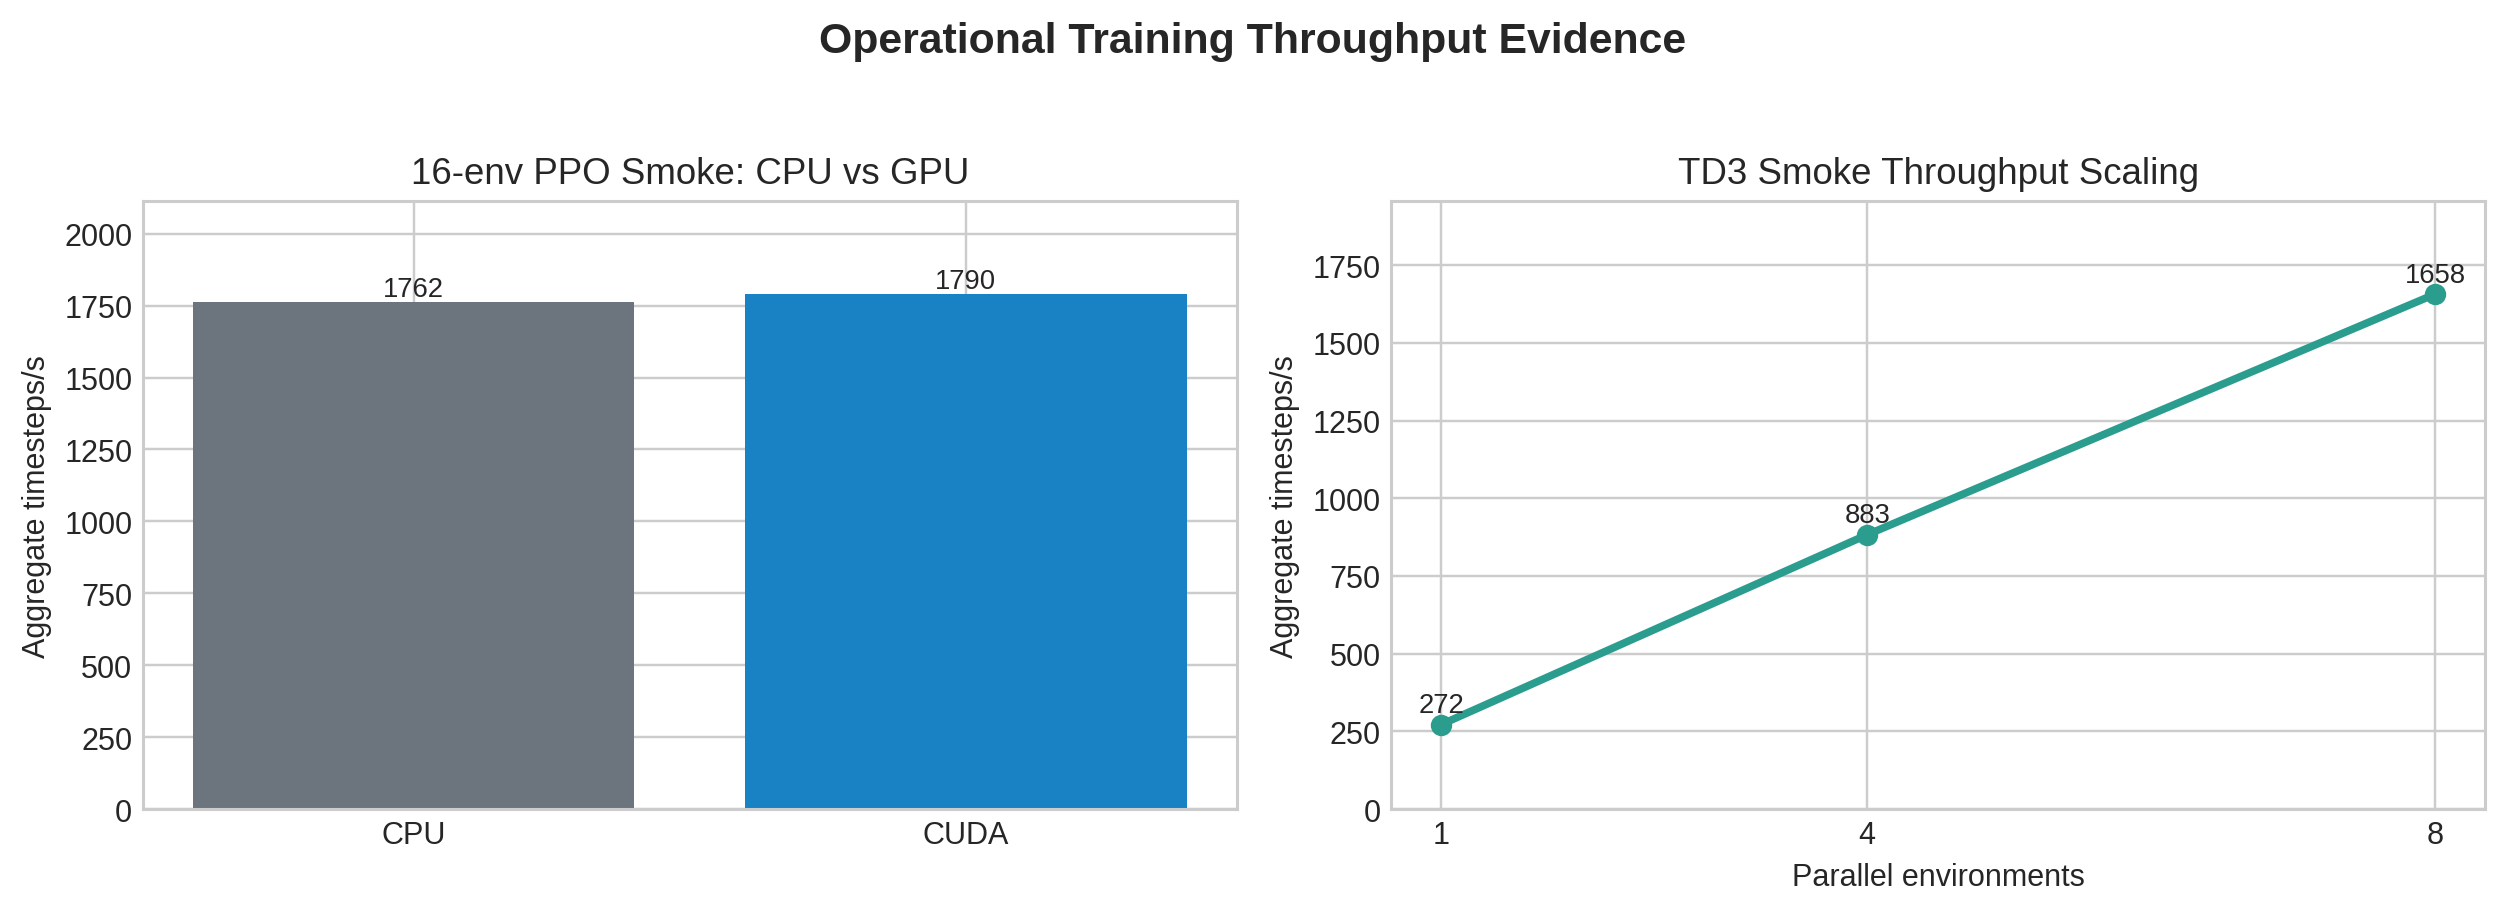
\includegraphics[width=\textwidth]{figures/phase1_throughput.png}
  \caption{Throughput evidence from the current kinematic training stack.}
\end{figure}

\section{Experimental Progress}

\subsection{Approach Policy Results}

\begin{table}[H]
\centering
\begin{tabularx}{\textwidth}{>{\raggedright\arraybackslash}p{0.25\textwidth} c c c c}
\toprule
Run & Success rate & Near-goal hit & Mean min pos. err. (m) & Avg. action mag. \\
\midrule
Previous best dwell5 & 0.72 & 0.77 & 0.0246 & 0.9405 \\
Balanced best20 & 0.71 & 0.74 & 0.0246 & 0.9337 \\
Balanced final long run & 0.28 & 0.46 & 0.0335 & 0.7987 \\
\bottomrule
\end{tabularx}
\caption{Representative approach-policy evaluation on 100 episodes.}
\end{table}

The main conclusion is that the approach skill itself is already learnable. The best checkpoints consistently reach roughly 71\%--72\% success on the evaluation suite. However, the final balanced long run fell to 28\%, which suggests that longer fine-tuning under handoff-oriented constraints can degrade the previously stable reaching behavior.

\subsection{Dock Policy Results}

\begin{table}[H]
\centering
\begin{tabularx}{\textwidth}{>{\raggedright\arraybackslash}p{0.28\textwidth} c c c c}
\toprule
Run & Strict success & Dwell success & Mean final pos. err. (m) & Regression rate \\
\midrule
Strict V2 mid & 0.23 & 0.58 & 0.0169 & 0.34 \\
Strict V2 long latest & 0.44 & 0.74 & 0.0132 & 0.27 \\
\bottomrule
\end{tabularx}
\caption{Representative dock-policy evaluation.}
\end{table}

The dock controller is improving, especially in local precision control. The long V2 checkpoint reached 44\% strict success and 74\% dwell success, which indicates that the dock stage is becoming usable as a local precision module, even though it is not yet robust enough for reliable full-pipeline switching.

\subsection{Switching and Joint Integration Results}

\begin{table}[H]
\centering
\begin{tabularx}{\textwidth}{>{\raggedright\arraybackslash}p{0.33\textwidth} c c c c}
\toprule
Experiment & Episodes & Near-goal entry & Overall success & Key observation \\
\midrule
Switched integration smoke & 5 & 0.40 & 0.00 & Switching can trigger in limited cases; 2 switch confirmations observed. \\
Switched integration full suite & 50 & 0.00 & 0.00 & Full handoff failed; no confirmed switch events. \\
Joint fine-tune smoke, approach branch & 50 & 0.00 & 0.00 & Approach collapsed after alternating fine-tuning. \\
Joint fine-tune smoke, dock branch & 50 & --- & 0.56 strict & Dock improved locally, but the pair is unbalanced. \\
\bottomrule
\end{tabularx}
\caption{Current integration status. The isolated modules are progressing, but the combined system is not yet stable.}
\end{table}

\begin{figure}[H]
  \centering
  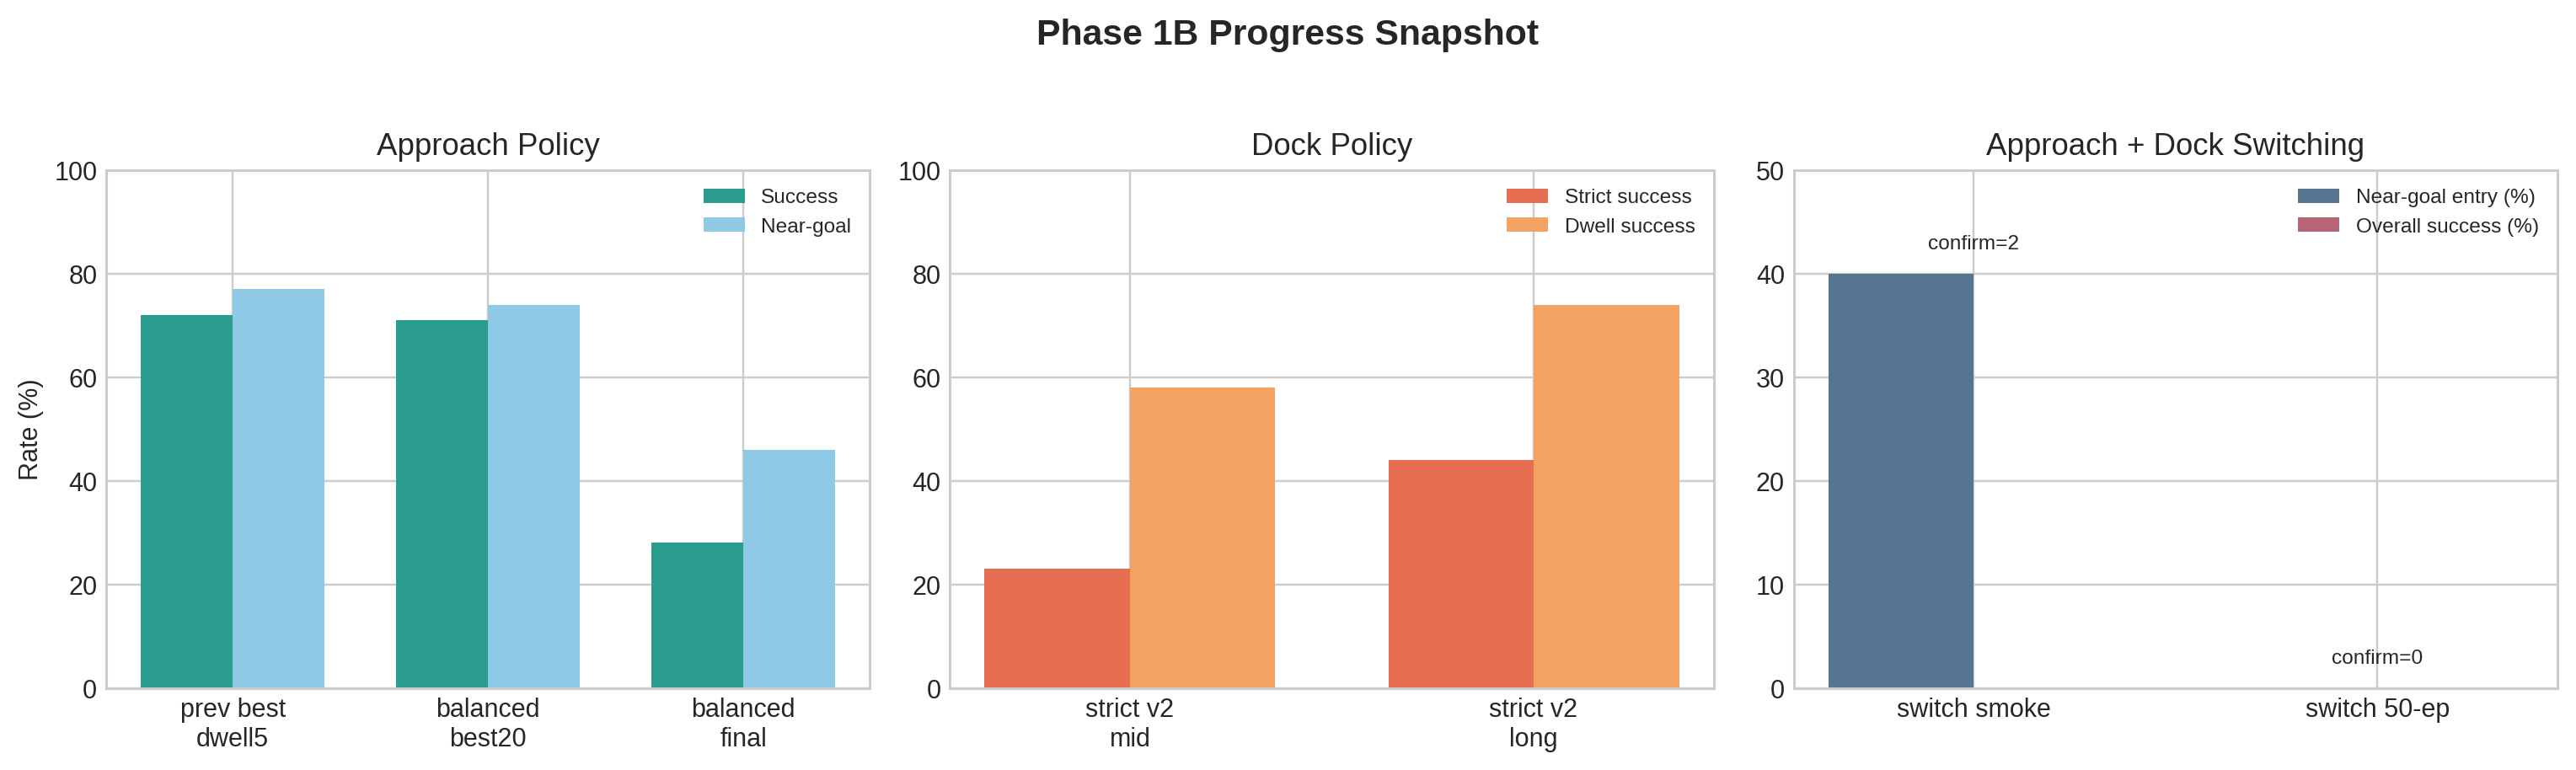
\includegraphics[width=\textwidth]{figures/phase1_progress_bars.png}
  \caption{Current progress snapshot across approach, dock, and switched integration experiments.}
\end{figure}

These results are the clearest reason we consider the project only about halfway complete. The individual modules work well enough to justify the architecture, but the handoff between them remains the main bottleneck.

\section{Interpretation of Current Progress}

The current experimental picture is internally consistent:
\begin{itemize}[leftmargin=1.5em]
  \item The \textbf{environment and tooling are working}. We can train, resume, benchmark, test, and evaluate in a reproducible way.
  \item The \textbf{approach policy is partially solved}. We already have checkpoints above 70\% success.
  \item The \textbf{dock policy is promising but not solved}. It shows useful local precision, but strict success is still below what we need for robust deployment.
  \item The \textbf{integration problem is still open}. The switched controller does not yet transfer consistently from approach into dock on the full evaluation suite.
  \item The \textbf{VLM part has not started}. We deliberately kept the scope focused on the kinematic RL foundation first.
\end{itemize}

Therefore, the project has a strong Phase 1 foundation, but it is not close to final completion. The main remaining work is not infrastructure anymore; it is the policy handoff and end-to-end robustness.

\section{What Remains for Phase 2}

The most important next steps are:
\begin{enumerate}[leftmargin=1.5em]
  \item Recover a stable approach policy under handoff-ready constraints.
  \item Improve the handoff distribution match between the end of approach and the start of docking.
  \item Tune the switching thresholds so that dock activation happens reliably without premature switching.
  \item Re-run alternating fine-tuning only after the approach branch stops collapsing.
  \item Start the VLM module only after the kinematic control backbone is stable enough to support it.
\end{enumerate}

\section{Conclusion}

At this Phase 1 checkpoint, the project is on track but not yet complete. The simulation, training, and evaluation foundation is operational. We have meaningful progress on both the approach and docking sub-problems, but the combined approach--dock pipeline is still the primary unresolved issue. The VLM component has not begun, and that is intentional at this stage. Overall, this is the correct point to classify the project as roughly halfway done: the foundation is real and working, but the final integrated behavior is not solved yet.

\appendix
\section{Packaged Evidence}

This submission package includes the following evidence files:
\begin{itemize}[leftmargin=1.5em]
  \item \texttt{evidence/approach\_eval\_100\_comparison.json}
  \item \texttt{evidence/dock\_eval\_100\_comparison.json}
  \item \texttt{evidence/switched\_eval\_summary\_smoke.json}
  \item \texttt{evidence/switched\_eval\_summary\_full.json}
  \item \texttt{evidence/joint\_training\_summary\_smoke.json}
  \item \texttt{evidence/phase1\_16env\_cpu\_vs\_gpu.json}
  \item \texttt{evidence/phase1\_parallel\_td3\_smoke.json}
  \item \texttt{evidence/kinematic\_tests\_20260422.txt}
  \item \texttt{evidence/jointprep\_pipeline\_log\_excerpt.txt}
\end{itemize}

\end{document}
